\documentclass{beamer}
%\usetheme{JLTree}

\usepackage{graphicx}
\usepackage[english]{babel}
\usepackage[latin1]{inputenc}
\usepackage[T1]{fontenc}
\usepackage{amsfonts}
\usepackage{url}
\usepackage{amsmath, amssymb, amsthm}
\usepackage{multicol}



\newcommand{\numberset}{\mathbb}
\newcommand{\N}{\numberset{N}}
\newcommand{\R}{\numberset{R}}
\newcommand{\Z}{\numberset{Z}}
\newcommand{\pscal}{\text{\large{\textbf{\textperiodcentered}}}}






% opening
\title[Optimization in Virtual Machine Networking]{Optimizations in Virtual Machine Networking}
\author[\hspace{2em} Vincenzo Maffione\hspace{3.6cm} Tesi di Laurea Magistrale \hspace{2.5cm} 27 Febbraio 2013]{}
\date{}


\begin{document}


\begin{frame}
\vspace*{-0.1cm}
\titlepage
\vspace*{-2.6cm}

\begin{center}
{\footnotesize Tesi di Laurea Magistrale\\
    Universit� di Pisa}
    \end{center}

    \begin{center}
    \begin{tabular}{l p{2.5cm} r c}

    \footnotesize\textsc{Relatore} & & \footnotesize\textsc{Candidato} \\
{\small Prof. \textit{Luigi Rizzo}} & &\small\textit{Vincenzo Maffione}\\
    \vspace{0.4em}
{\footnotesize Universit� di Pisa} & &\\
	\footnotesize\textsc{Correlatore} & &  \\
{\small Prof. \textit{Giuseppe Lettieri}} && \\
{\footnotesize Universit� di Pisa} && \\
    \end{tabular}
    \end{center}

    \begin{center}
{\small 27 Febbraio 2013}
\end{center}

\end{frame}



\begin{frame}
  \begin{block}{Goals}
    \begin{itemize}
      \item Analyze the state of the art in Virtual Machines networking, when hardware based virtualization is employed
      \item Implement optimizations aimed at improving the Rx/Tx packet rate when a virtual e1000 network adapter is used in a Virtual Machine
    \end{itemize}

  \end{block}
\end{frame}

%=================================================================
\section{Introduction}
%=================================================================

\begin{frame}
\frametitle{Introduction}

  \only<1> {
  \begin{block}{What is a Virtual Machine?}
    \begin{itemize}
      \item A protected execution environment able to execute code under the control of an \emph{hypervisor} (or
	    \emph{Virtual Machine Monitor})
      \item Several Virtual Machines (\emph{guests}) can be run on a single physical machine (\emph{host})
    \end{itemize}

  \end{block}
  }
 
  \only<2> {
  \begin{block}{Virtual Machine Systems}
    \begin{itemize}
      \item Used to build systems more complex than the standard three-layers computer systems
      \item Very powerful tools
      \item Widely employed in data centers and organizations
      \item Easy to use also for inexperienced users
      \item VM technologies are constantly changing
    \end{itemize}
  \end{block}
  }

  \only<3> {
  \begin{block}{Virtual Machines advantages}
    \begin{itemize}
      \item Flexibility
      \item Protection
      \item Improved resource usage
      \item Mobility
    \end{itemize}
  \end{block}
  }
 
  \only<4> {
  \begin{block}{Virtual Machines classification}
    \begin{itemize}
      \item Process VMs
	\begin{itemize}
	  \item Same ABI (multiprogramming)
	  \item Different ABI (High level language interpreters, binary translators)
	\end{itemize}

      \item System VMs
	\begin{itemize}
	  \item Same ISA (Type 1 VMM or Type 2 VMM)
	  \item Different ISA (System emulators)
	\end{itemize}

    \end{itemize}
  \end{block}
  }

  \only<5> {
  \begin{figure}[ht]
	\begin{minipage}[b]{0.45\linewidth}
	\centering
	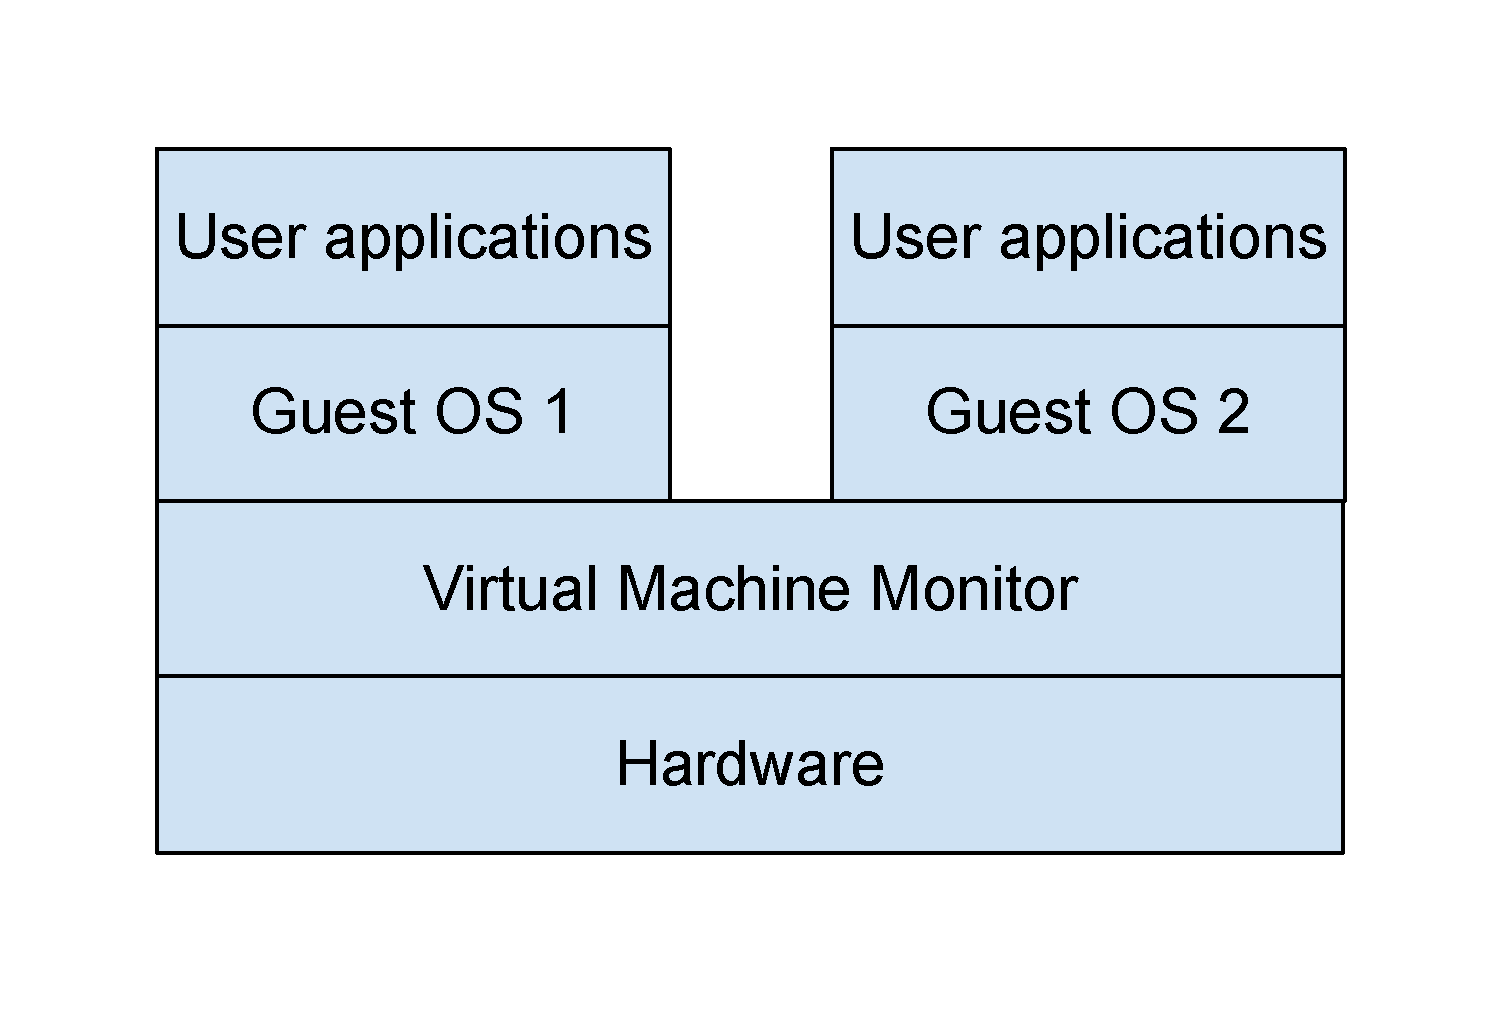
\includegraphics[width=\textwidth]{type-1-vmm.pdf}
	\caption{Type 1 VMM example}
	\label{fig:figure1}
	\end{minipage}
	\hspace{0.5cm}
	\begin{minipage}[b]{0.45\linewidth}
	\centering
	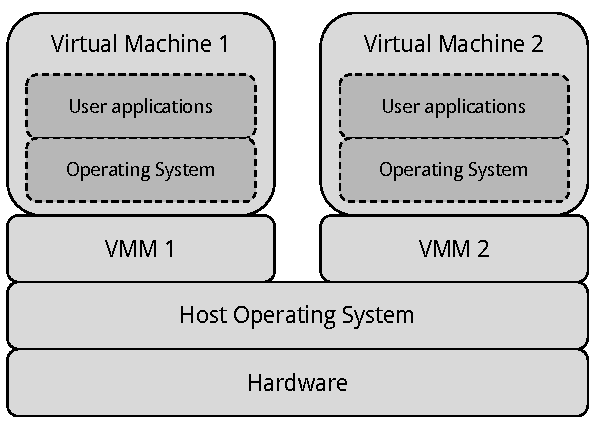
\includegraphics[width=\textwidth]{type-2-vmm.pdf}
	\caption{Type 2 VMM example}
	\label{fig:figure2}
	\end{minipage}
  \end{figure}
  }
  
  \only<6> {
  \begin{block}{CPU Virtualization techniques}
    \begin{itemize}
      \item Interpretation: Doing in software what a CPU does in hardware
      \item Binary translation: Translating the guest code in equivalent host code \emph{on the fly}
      \item Hardware assisted CPU virtualization: Using processor extensions such as Intel VT-x or AMD-v
    \end{itemize}
  \end{block}
  }
\end{frame}



%=================================================================
\section{Working environment}
%=================================================================

\begin{frame}
\frametitle{Our reference hypervisor}

  \begin{block}{QEMU-KVM}
    \begin{itemize}
      \item Free, open source and multi-platform system emulator
      \item Type 2 VMM $\longrightarrow$ a VM is a process in the host OS
      \item Can make use of Kernel-based Virtual Machine (KVM) for native guest code execution
      \item Emulates SMP systems
      \item Also supports Process VMs (using binary translation)
    \end{itemize}
  \end{block}
\end{frame}


\begin{frame}
\frametitle{QEMU-KVM internal structure}

  \only<1> {
  \begin{block}{Threads of a QEMU process}
      \begin{itemize}
	\item Event-loop based
	\item A thread for each guest VCPU
	\item A dedicated \emph{IOThread} executes the event-loop
	\item The IOThread lets the guest communicate with the outside world
      \end{itemize}
    \end{block}
  }
  
  \only<2> {
    \begin{figure}
    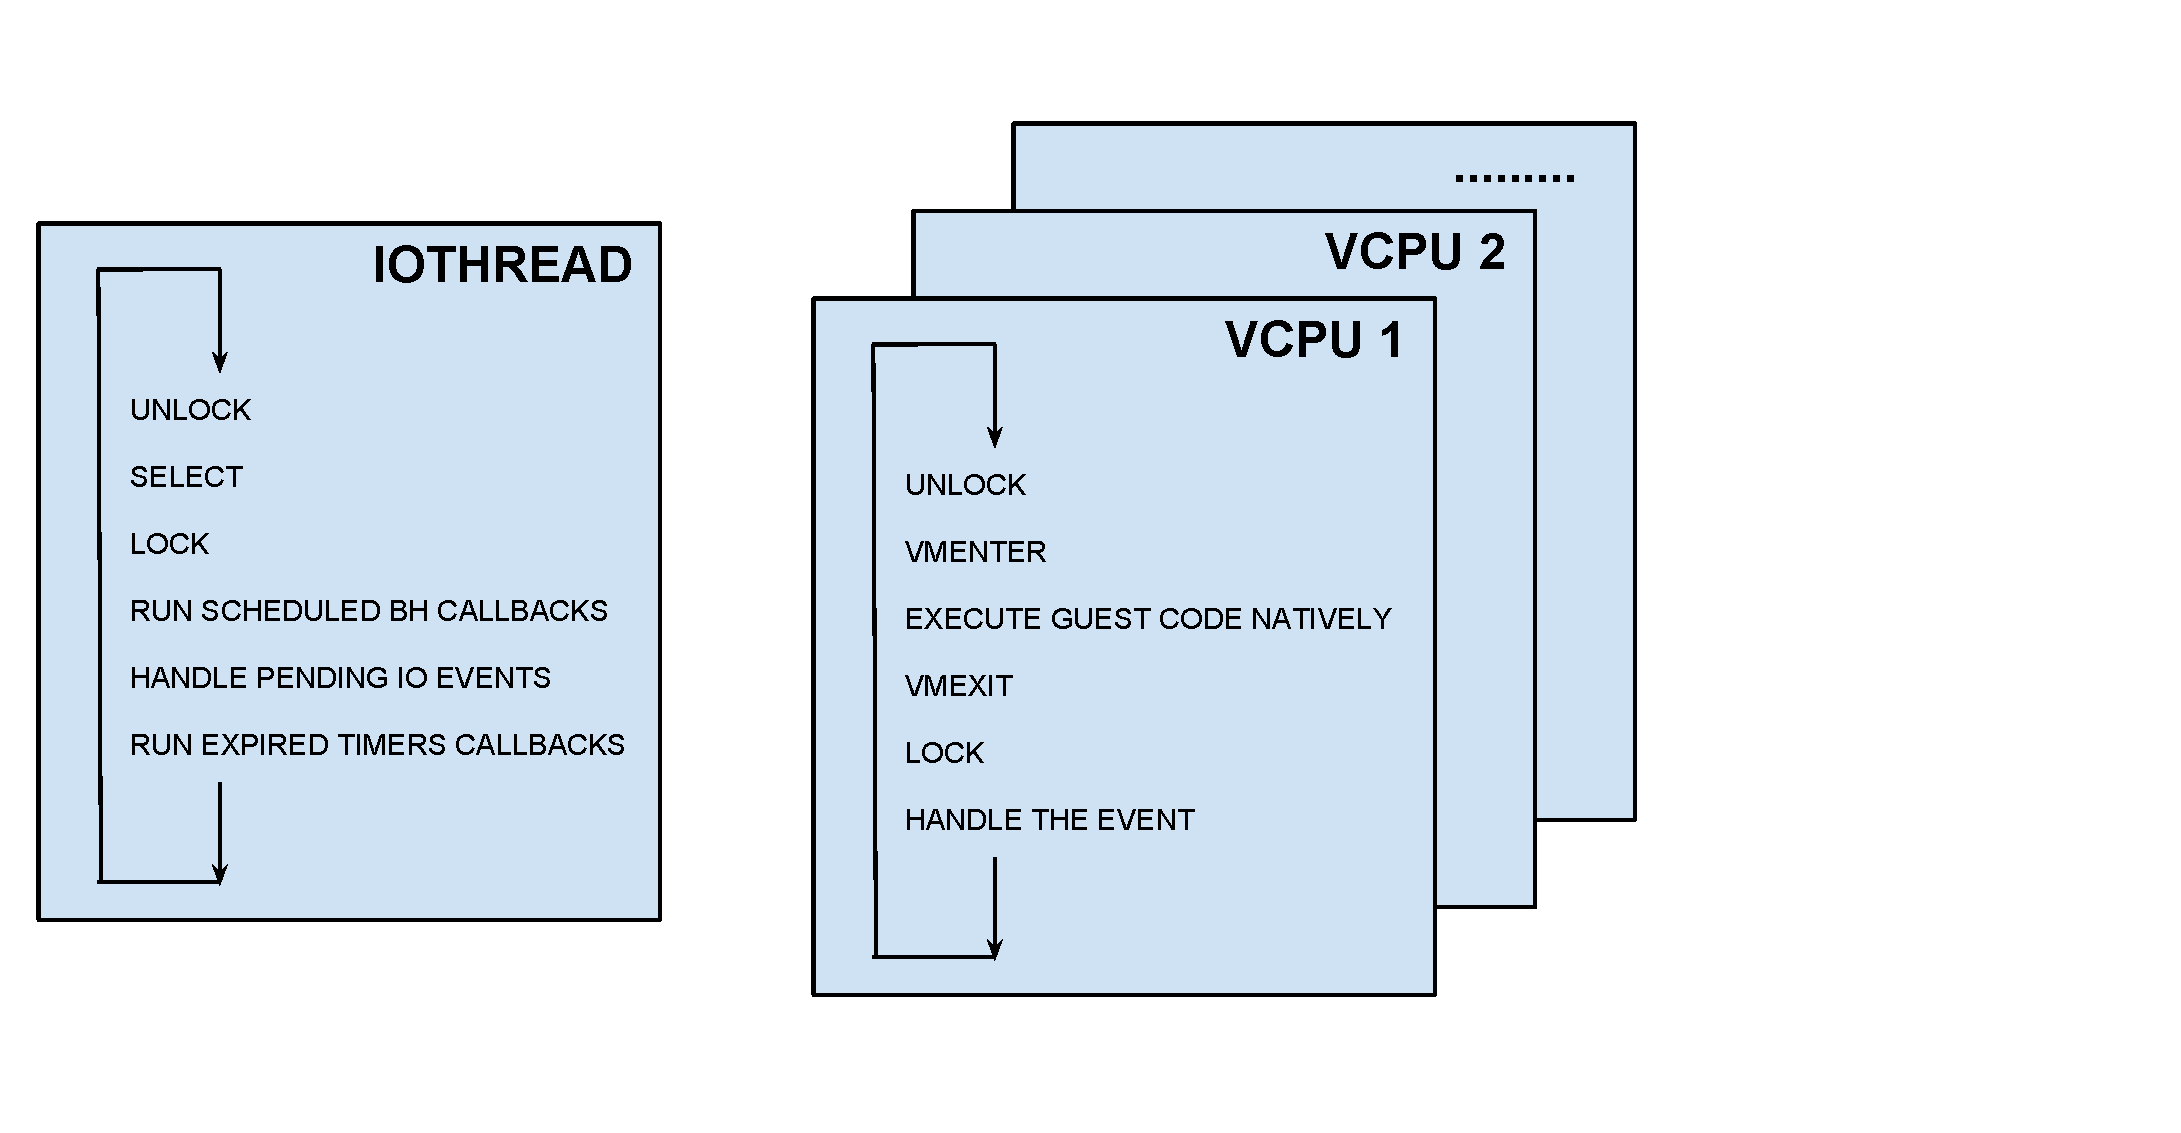
\includegraphics[width=.80\columnwidth]{qemu-threads.pdf}
    \end{figure}
  }
  
  \only<3> {
    \begin{block}{KVM mechanics}
      \begin{itemize}
	\item With KVM, VCPUs switch between guest world and host world
	\item A switch occurs when the VCPU tries to access the I/O space, MMIO or when it receives an interrupt
	\item The hypervisor can \emph{inject} interrupts into the guest
	\item I/O emulation can be done both by VCPUs (when in the host world) and by IOThread
	\item Mutual exclusion required $\longrightarrow$ A \emph{Big-Lock} is employed
      \end{itemize}
    \end{block}
  }
\end{frame}

    
\begin{frame}
  \frametitle{QEMU networking}
  \only<1> {
  \begin{block}{Need for networking support}
      \begin{itemize}
	\item A VM is almost useless if isolated from the outside world 
	\item Guest OS thinks to deal with a physical network adapter, and uses the original driver
	\item The network adapter is emulated by a QEMU \emph{network frontend}
	\item A QEMU \emph{network backend} provides connectivity to the outside world
	\item Frontend and backend exchange network packets
      \end{itemize}
    \end{block}
  }
  
  \only<2> {
    \begin{figure}
    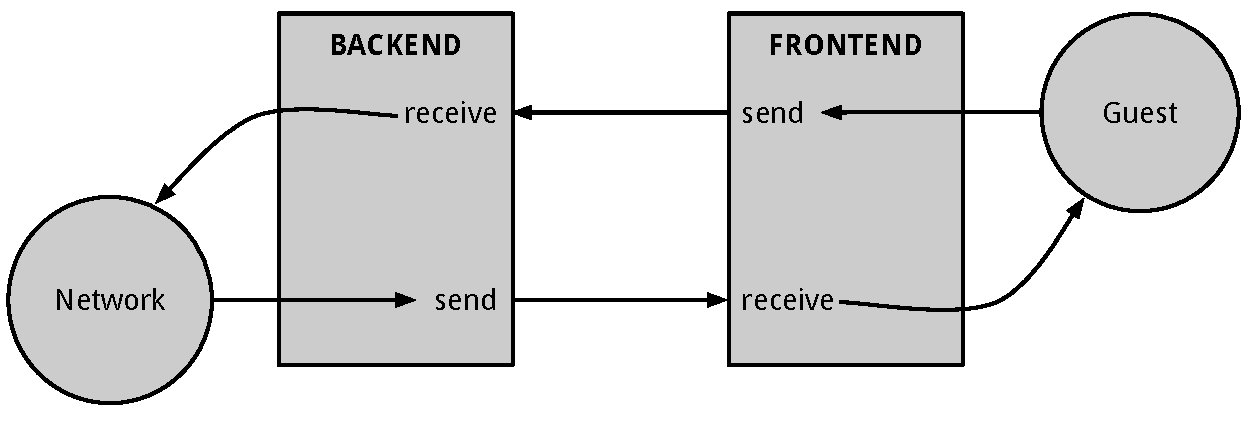
\includegraphics[width=.90\columnwidth]{frontend-backend.pdf}
    \end{figure}
  }
  
  \only<3> {
  \begin{block}{What we have chosen to address for our optimizations}
      \begin{itemize}
	\item The e1000 network adapter, emulated in virtually all emulators
	\item The TAP backend, implemented using TAP devices
	\item A TAP device is associated to one and only one network adapter
	\item Many TAP devices can be bridged together, in order to emulate a LAN of VMs
      \end{itemize}
    \end{block}
  }
  
  \only<4> {
    \begin{figure}
      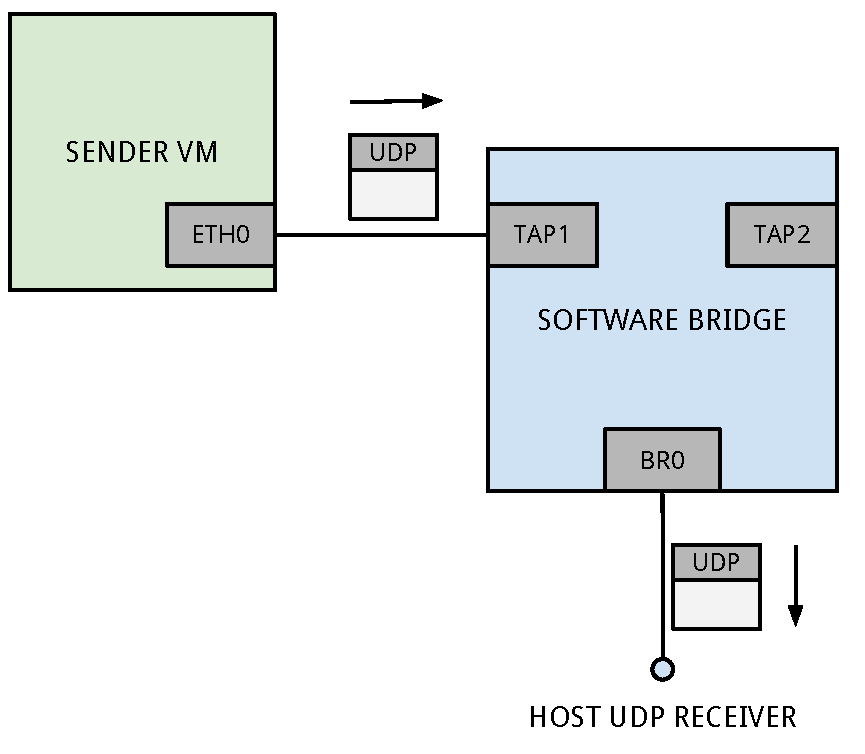
\includegraphics[width=.55\columnwidth]{scenario-1.pdf}
      \caption{An example of a system with a VM connected to a TAP backend}
    \end{figure}
  }
\end{frame}


\begin{frame}
\frametitle{The e1000 interface specification}
  \only<1> {
    \begin{block}{How do driver and device exchange packets?}
      \begin{itemize}
	\item Two array of descriptors (\emph{rings}) are used to exchange address/length pairs: TX ring and RX ring
	\item Each address/length pair references a buffer to send (TX ring) or a buffer to receive into (RX ring)
	\item The driver inserts descriptors to give buffers to the device
	\item The device uses the buffers and gives them back to the driver
	\item Synchronization is achieved using head/tail index registers
      \end{itemize}
    \end{block}
  }
  
  \only<2> {
    \begin{figure}
      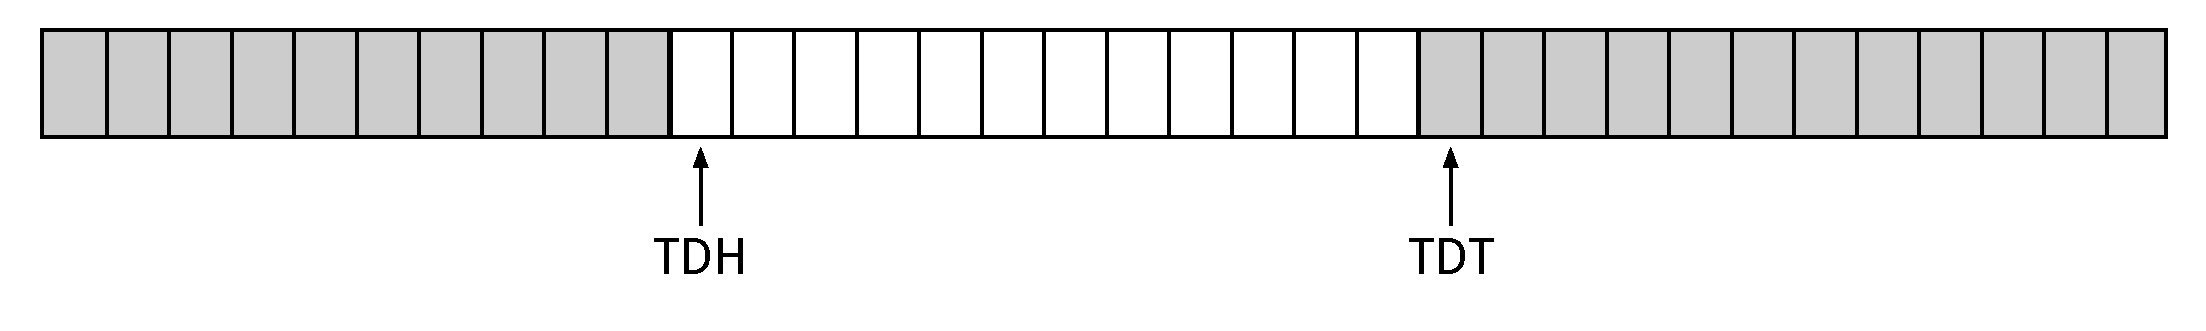
\includegraphics[width=.95\columnwidth]{tx-ring.pdf}
      \caption{TX ring}
    \end{figure}
    \begin{figure}
      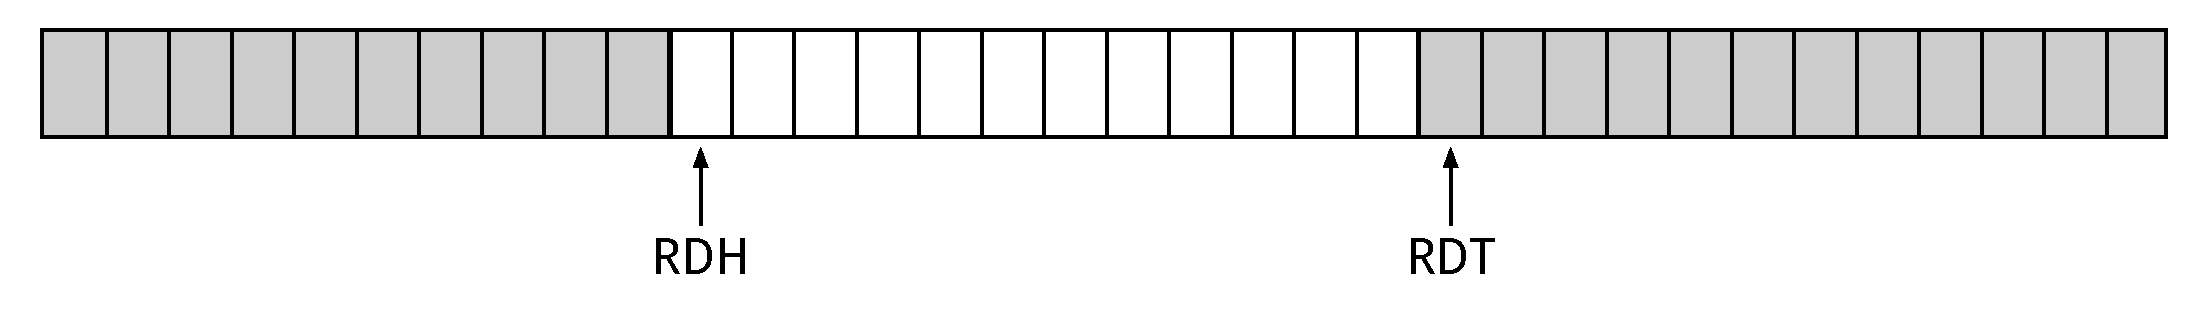
\includegraphics[width=.95\columnwidth]{rx-ring.pdf}
      \caption{RX ring}
    \end{figure}
  }
\end{frame}


\begin{frame}
\frametitle{QEMU e1000 emulation}
  \begin{block}{How is emulation performed?}
    \begin{enumerate}
      \item The VCPU tries to access an e1000 register $\rightarrow$ The processor switches to the host world (exits), yielding the 
	    control to QEMU
      \item QEMU analyzes the exit reason and invokes the associated callback
      \item The callback (e1000 frontend) emulates all the side effects of the register access
      \item The VCPU switch back to (enters) the guest world
    \end{enumerate}
  \end{block}
\end{frame}
   
    
\begin{frame}
\frametitle{Linux e1000 device driver}
  \only<1> {
    \begin{block}{Interface with the Linux network stack on the TX path}
      \begin{itemize}
	\item A Linux process wants to send a packet $\rightarrow$ the kernel invokes the e1000 \texttt{ndo\_start\_xmit()} method
	\item The driver inserts a new TX descriptor in the ring and updates the TDT register
      \end{itemize}
    \end{block}
  
    \begin{block}{Interface with the Linux network stack on the RX path}
      \begin{itemize}
	\item The adapter receives a packet into the RX ring $\rightarrow$ An interrupt is raised
	\item The driver interrupt routine pushes the receive packet to the network stack (\texttt{netif\_rx()})
      \end{itemize}
    \end{block}
  }
  
  \only<2> {
    \begin{figure}
      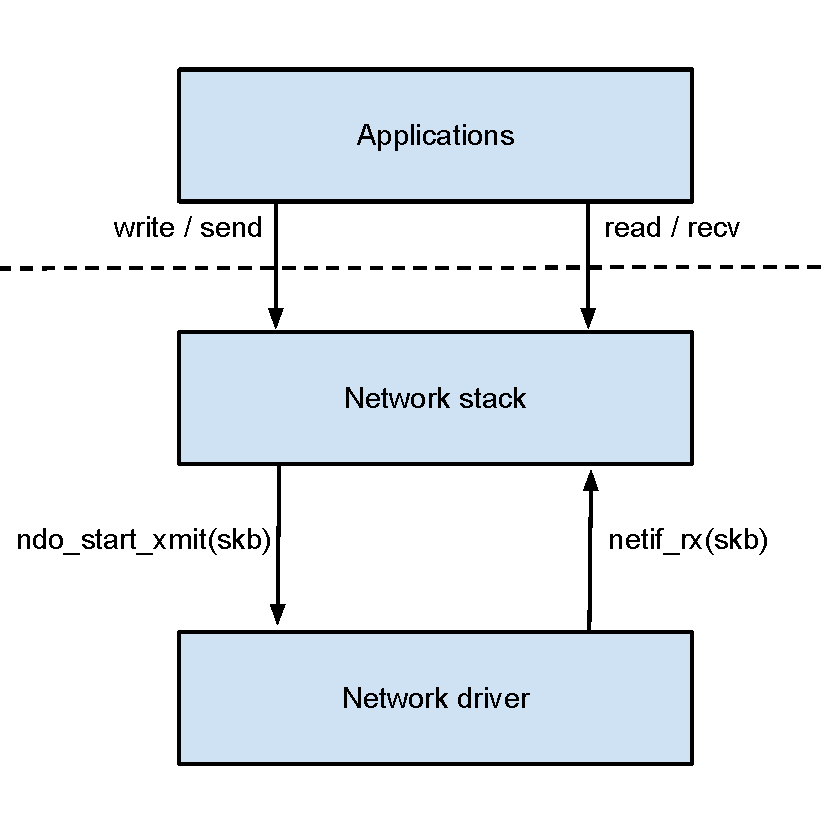
\includegraphics[width=.55\columnwidth]{linux-interface.pdf}
    \end{figure}
  }
\end{frame}



%=================================================================
\section{e1000 optimizations}
%=================================================================

\begin{frame}
\frametitle{Problems of the existing implementation}

  \only<1> {
    \begin{block}{TX statistics}
    \begin{center}
    \begin{tabular}{lrl}
      \textbf{Interrupt rate} & 20.567 & KHz\\
      \textbf{TX packet rate} & 20.567 & Kpps\\
      \textbf{TX notifications rate} & 20.567 & KHz\\
      \textbf{MMIO write rate} & 61.702 & KHz\\
      \textbf{MMIO read rate} & 61.702 & KHz\\
    \end{tabular}
    \end{center}
    \end{block}
  }
  
  \only<2> {
    \begin{block}{RX statistics}
    \begin{center}
    \begin{tabular}{lrl}
      \textbf{Interrupt rate} & 14.314 & KHz\\
      \textbf{RX packet rate} & 14.403 & Kpps\\
      \textbf{RX notifications} & 14.288 & Mbps\\
      \textbf{MMIO write rate} & 42.861 & KHz\\
      \textbf{MMIO read rate} & 42.860 & KHz\\
    \end{tabular}
    \end{center}
    \end{block}
  }

  \only<3> {
    \begin{block}{What are the problems and bottlenecks?}
      \begin{itemize}
	\item Interrupt mitigation is not emulated, although present in the real hardware $\rightarrow$ We get an interrupt for each
	      TX or RX packet
	\item 5 register accesses in the interrupt routine
	\item A TX notification for each TX packet
	\item A RX notification for each RX packet
	\item Interrupts and register accesses are extremely expensive
	\item Moreover, TX emulation is done synchronously $\rightarrow$ Parallelism is affected
      \end{itemize}
    \end{block}
  }
\end{frame}


\begin{frame}
\frametitle{Adding interrupt moderation}
  \only<1> {
    \begin{block}{Interrupt moderation patch}
      \begin{itemize}
	\item The e1000 frontend limits the Maximum Interrupt Rate $\rightarrow$ Interrupts are coalesced
	\item To achieve that, we use a timer to delay the interrupts
	\item The patch is only 50 lines of code
      \end{itemize}
    \end{block}
    }
    
    \only<2> {
    \begin{block}{TX statistics improvements}
      \begin{center}
      \begin{tabular}{lrcrl}
      \textbf{Interrupt rate} & 20.567 & $\rightarrow$ & 3.805 & KHz\\
      \textbf{TX packet rate} & 20.567 & $\rightarrow$ & 47.849 & Kpps\\
      \textbf{TX notifications rate} & 20.567 & $\rightarrow$ & 47.849 & KHz\\
      \textbf{MMIO write rate} & 61.702 & $\rightarrow$ &55.464 & KHz\\
      \textbf{MMIO read rate} & 61.702 & $\rightarrow$ & 11.478 & KHz\\
      \end{tabular}
      \end{center}
    \end{block}
    }
    
    \only<3> {
    \begin{block}{RX statistics improvements}
      \begin{center}
      \begin{tabular}{lrcrl}
	\textbf{Interrupt rate} & 14.314 & $\rightarrow$ & 3.838 & KHz\\
	\textbf{RX packet rate} & 14.403 & $\rightarrow$ & 137.103 & Kpps\\
	\textbf{RX notifications} & 14.288 & $\rightarrow$ & 10.322 & Mbps\\
	\textbf{MMIO write rate} & 42.861 & $\rightarrow$ & 17.990 & KHz\\
	\textbf{MMIO read rate} & 42.860 & $\rightarrow$ & 11.502 & KHz\\
      \end{tabular}
      \end{center}
    \end{block}

    }
\end{frame}


\begin{frame}
\frametitle{Moderating TX notifications}
    \only<1> {
    \begin{block}{TDT \emph{write batching} patch}
      \begin{itemize}
	\item The e1000 driver coalesces TX notifications
	\item This is done without using expensive kernel timers
	\item We don't notify if there is a pending TX interrupt
	\item We use the e1000 interrupt routine to flush pending TX frames
	\item The patch is only 35 lines of code
      \end{itemize}
    \end{block}
    }
    
    \only<2> {
    \begin{block}{TX statistics improvements w.r.t. moderation patch statistics}
      \begin{center}
      \begin{tabular}{lrcrl}
      \textbf{Interrupt rate} & 3.805 & $\rightarrow$ & 1.848 & KHz\\
      \textbf{TX packet rate} & 47.849 & $\rightarrow$ & 163.519 & Kpps\\
      \textbf{TX notifications rate} & 47.849 & $\rightarrow$ & 1.847 & KHz\\
      \textbf{MMIO write rate} & 55.464 & $\rightarrow$ & 5.546 & KHz\\
      \textbf{MMIO read rate} & 11.478 & $\rightarrow$ & 5.605 & KHz\\
      \end{tabular}
      \end{center}
    \end{block}
    }
\end{frame}



%=================================================================
\section{A paravirtualized e1000}
%=================================================================

\begin{frame}
\frametitle{The paravirtualization concept}
  \only<1> {
    \begin{block}{Full virtualization}
      \begin{itemize}
	\item So far we have assumed that the guest OS is completely unaware of being run in a Virtual Machine environment
	\item This type of virtualization is called \emph{Full virtualization}
	\item Advantage: The hypervisor can support an unmodified OS
	\item Disadvantage: Hypervisor implementation is generally complicated and inefficient
      \end{itemize}
    \end{block}
  }
  
  \only<2> {
    \begin{block}{Paravirtualization}
      \begin{itemize}
	\item The guest OS is aware of being under the control of an hypervisor
	\item Guest and hypervisor can communicate in a simpler and more efficient way
	\item MMIO accesses and interrupts are used \emph{only} for notifications and never to exchange data
	\item Data are exchanged only through shared memory
      \end{itemize}
    \end{block}
  }
\end{frame}

\begin{frame}
\frametitle{The Virtio standard}

  \only<1> {
    \begin{block}{Virtio}
      \begin{itemize}
	\item A de-facto standard for I/O paravirtualization
	\item A set of new efficient device drivers/emulators
	\item Increase code reuse across devices and platforms
      \end{itemize}
    \end{block}
  }
  
  \only<2> {
    \begin{figure}
      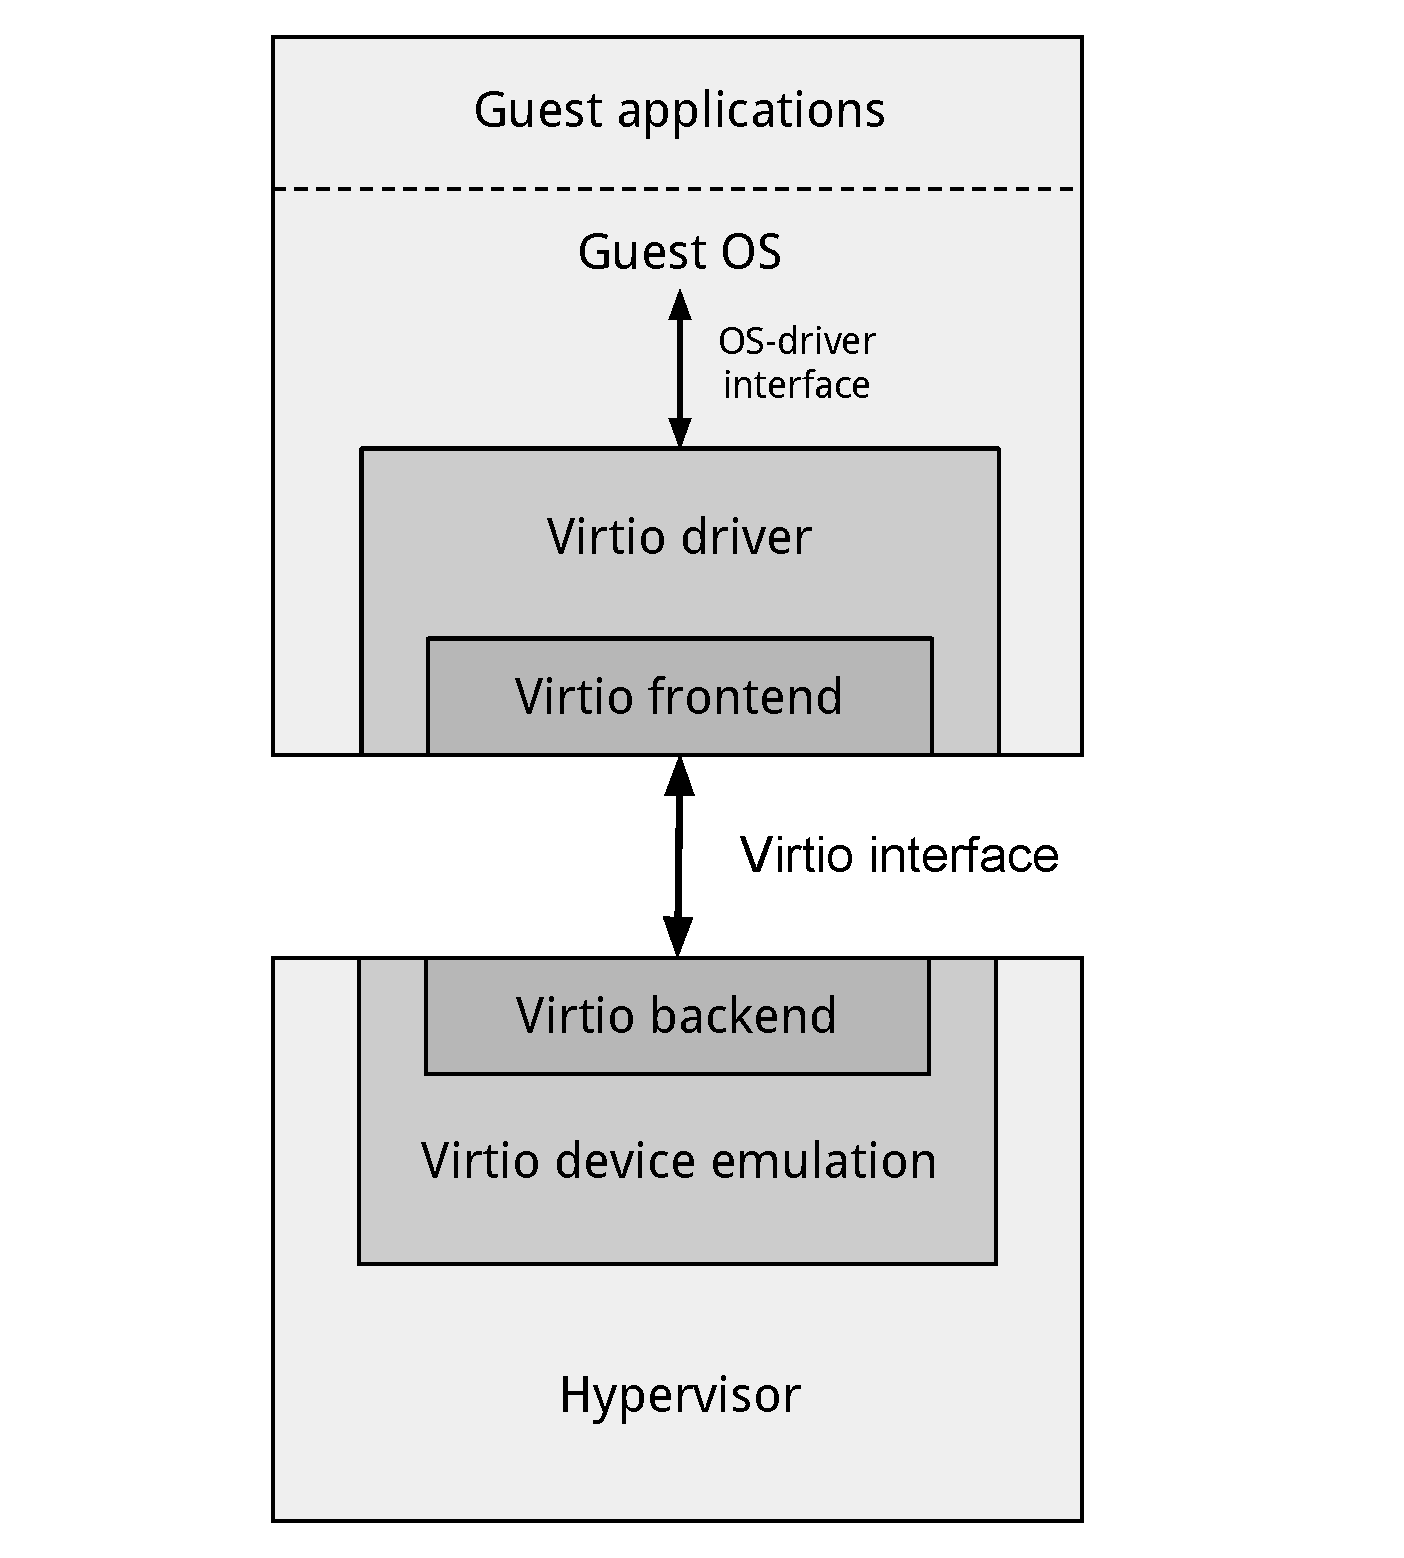
\includegraphics[width=.55\columnwidth]{virtio.pdf}
    \end{figure}
  }
  
  \only<3> {
    \begin{figure}
      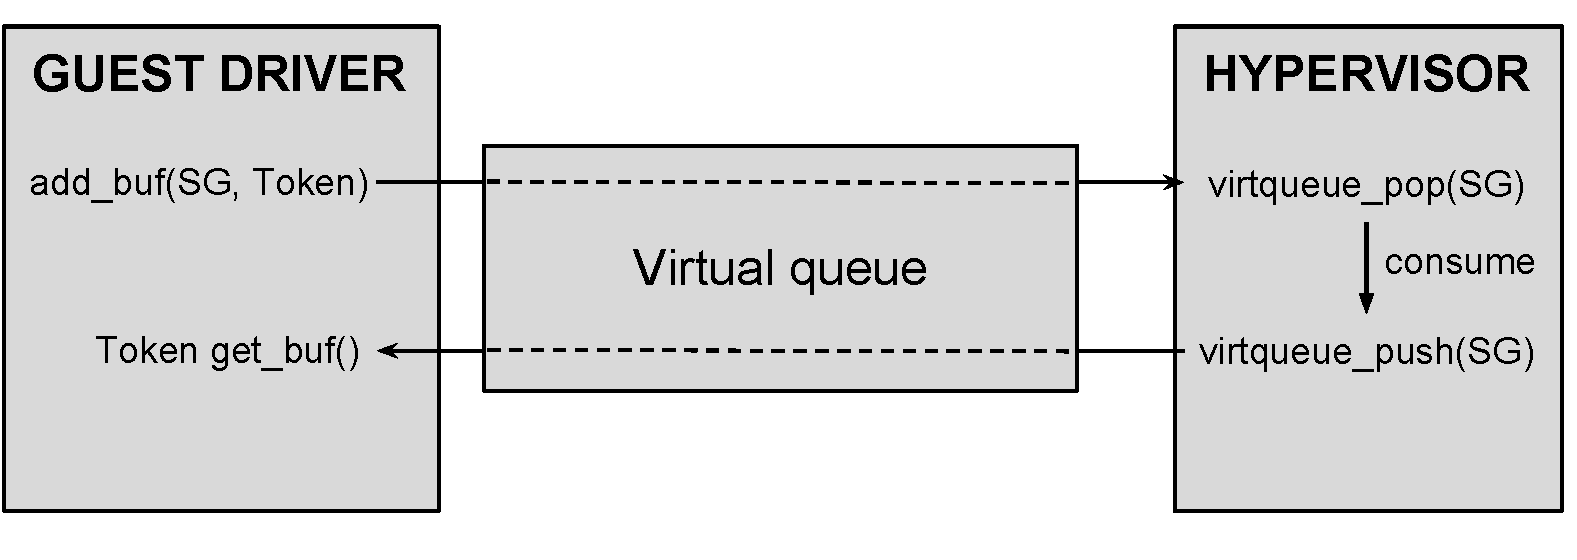
\includegraphics[width=.9\columnwidth]{virtqueue.pdf}
      \caption{Driver and hypervisor can exchange data through a virtual queue}
    \end{figure}
  }
\end{frame}


\begin{frame}
\frametitle{Porting the paravirtualization concept to e1000}

  \only<1> {
    \begin{block}{Notification-efficient producer/consumer communication}
      \begin{itemize}
	\item e1000 index registers exported to a shared memory area (\emph{Communication Status Block})
	\item Added flags to enable/disable TX/RX notifications
	\item Two Producer/consumer couples (PCCs) for the TX path and two PCCs for the RX path
	\item Consumer work is done asynchronously w.r.t. the producer and with notifications disabled
	\item The producer notifies the consumer only when the consumer stops
	\item If the consumer is faster notification moderation is required
      \end{itemize}

    \end{block}
  }
  
  \only<2> {
    \begin{block}{Paravirtualization patch}
      \begin{itemize}
	\item Both e1000 driver and e1000 must be patched
	\item About 100 lines of code in the hypervisor
	\item About 40 lines in the Linux kernel
      \end{itemize}
    \end{block}

  }
  
  \only<3> {
    \begin{block}{TX statistics improvements w.r.t. moderation patch statistics}
      \begin{center}
      \begin{tabular}{lrcrl}
      \textbf{Interrupt rate} & 3.805 & $\rightarrow$ & 0.370 & KHz\\
      \textbf{TX packet rate} & 47.849 & $\rightarrow$ & 183.447 & Kpps\\
      \textbf{TX notifications rate} & 47.849 & $\rightarrow$ & 0.438 & KHz\\
      \textbf{MMIO write rate} & 55.464 & $\rightarrow$ & 1.181 & KHz\\
      \textbf{MMIO read rate} & 11.478 & $\rightarrow$ & 0.430 & KHz\\
      \end{tabular}
      \end{center}
    \end{block}
  }
    
  \only<4> {
    \begin{block}{RX statistics improvements w.r.t. moderation patch statistics}
      \begin{center}
      \begin{tabular}{lrcrl}
	\textbf{Interrupt rate} & 3.838 & $\rightarrow$ & 3.774 & KHz\\
	\textbf{RX packet rate} & 137.103 & $\rightarrow$ & 317.335 & Kpps\\
	\textbf{RX notifications} & 10.322 & $\rightarrow$ & 0.002 & Mbps\\
	\textbf{MMIO write rate} & 17.990 & $\rightarrow$ & 7.358 & KHz\\
	\textbf{MMIO read rate} & 11.502 & $\rightarrow$ & 3.678 & KHz\\
      \end{tabular}
      \end{center}
    \end{block}
  }
  
\end{frame}


%=================================================================
\section{Conclusions and future work}
%=================================================================
\begin{frame}
\frametitle{Conclusions}
  \begin{block}{}
    \begin{itemize}
      \item Some simple modifications to the e1000 framework lead to big performance improvements
      \item TX path: $8.9\times$ speed-up
      \item RX path: $22\times$ speed-up
      \item Collecting the idea presented in this work, in combination with the VALE fast switch, we have submitted a short paper
	    to USENIX ATC'13
    \end{itemize}
  \end{block}
\end{frame}

\begin{frame}
\frametitle{Future works}
  \begin{block}{More can be done to optimize e1000 performance in VM systems}
    \begin{itemize}
      \item Remove redundant packet copies in the TX path
      \item Euristics to improve latency, byassing interrupt moderation
      \item Use emulated MSI/MSI-X interrupts
      \item Explore TSO/GSO to improve TCP throughput
    \end{itemize}
  \end{block}
\end{frame}


\begin{frame}
\begin{center}
{\Large The end}
\end{center}

\end{frame}
\end{document}
